
\section{Electromagnetic Calorimeter}

% AMS Electromagnetic Calorimeter
The ECAL in the AMS-02 experiment can precisely measure the longitudinal and lateral electromagnetic shower development and also the deposited energy \cite{ECALPaper1, ECALPaper2}. It has a lead-scintillating fiber sandwich structure with an active area of 648 $mm$ $\times$ 648 $mm$, a thickness of 166.5 $\rm{mm}$ and a weight of $\sim 500$ kg. The ECAL has 98 lead foils and 50000 scintillating fibers in total. The entire structure corresponds to 17 radiation lengths ($X_0$). \par

% Super Layer
The ECAL consists of 9 superlayers with a thickness of 18.5 mm each. Each superlayer is made of 11 grooved lead foils alternated with ten fiber layers glued together with optical epoxy (figure \ref{ECALSuperLayer}) \cite{ECALFibres}, while the last foil of the last superlayer is made of aluminum. In each superlayer, the fibers are oriented along one direction only. By alternatively stacking the nine superlayers in the X and Y directions  (five superlayers in the X direction and four in the Y direction), the 3D image of the shower shape is obtained. Each superlayer’s fibers are read out by 36 PMTs at only one end. In total, the ECAL has 324 PMTs \cite{ECALPaper3}.   \par

\begin{figure}[h]
\centering
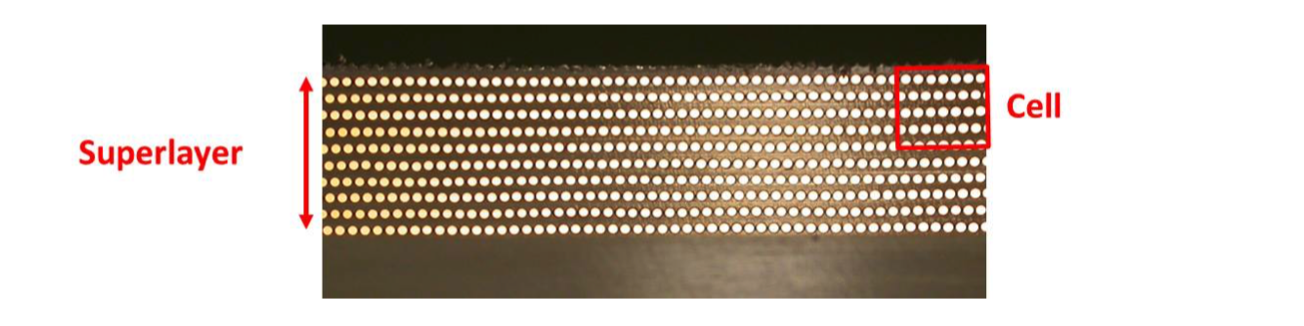
\includegraphics[width=1.0\textwidth, height=0.2\textheight ]{Figures/chapter3/ECAL/SuperLayer.png}
\caption[The ECAL superlayer structure.]{The ECAL superlayer structure. One cell is shown in red \cite{ECALPaper3}.}
\label{ECALSuperLayer}
\end{figure}

% ECAL Shower
When a particle goes through the ECAL, it interacts in an electromagnetic or hadronicdal way producing a shower \cite{ECALShowerPaper}. When an electron or positron traverses the ECAL, it emits photons by bremsstrahlung, then the emitted photons convert to electrons and positrons further by pair production, so a cascaded electromagnetic shower develops. While a proton or antiproton traverses the ECAL, it passes as a minimum ionizing particle (MIP) and leaves a relatively clear track. The produced hadronic shower primarily consists of pions and kaons which can interact or decay further. Due to the transverse momenta for massive secondaries and the possible production of neutral particles, the hadronic shower is wider and more irregular than the electromagnetic shower.  \par 

The different shower shapes can be used to distinguish between electrons and protons (antiprotons). Combined with the tracker measurement ($E/|R|$ cut), the ECAL provides a proton rejection power larger than $10^4$ at an electron efficiency of 90\% in the energy range of 3 to 1000 GeV. In figure \ref{ECALProtonRejectionPower}, the proton rejection of the ECAL is shown. \par


\begin{figure}[H] 
\centering   
\subfigure[] { \label{ECALProtonRejectionPower}    
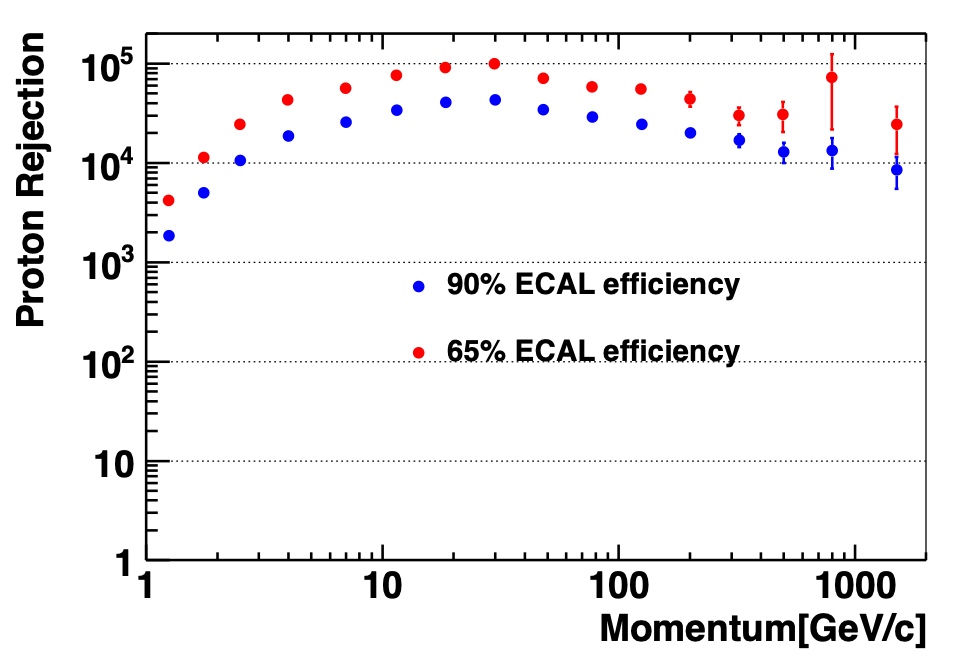
\includegraphics[width=0.45\columnwidth, height=0.225\textheight]{Figures/chapter3/ECAL/Ecal_Proton_Rejection.png} 
}    
\subfigure[] { \label{ECALEnergyResolution}    
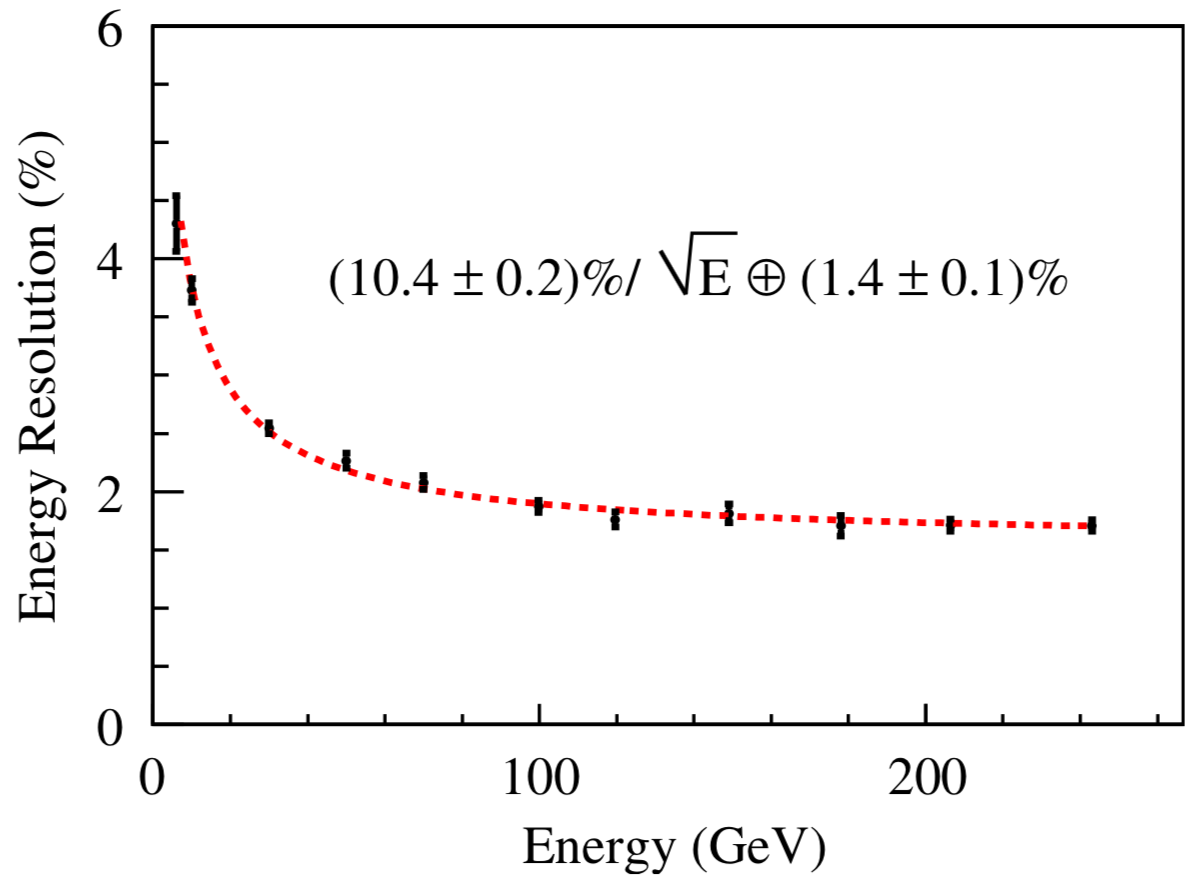
\includegraphics[width=0.45\columnwidth, height=0.225\textheight]{Figures/chapter3/ECAL/EnergyResolution.png}    
}     
\caption[The ECAL rejection power and energy resolution.]{a) The proton rejection of the ECAL at 65\% and 90\% electron efficiency \cite{AMSWebside}. b) The ECAL energy resolution determined from test beam data. The function of equation \ref{EcalResolutionEquation} is also shown (red dashed line) \cite{ECALResolution}.}
\end{figure}

% Resolution
The energy resolution has been determined in a CERN test beam \cite{ECALBeamTest} and can be described by \cite{ECALResolution}: 

\begin{equation}
\frac{\sigma (E)}{E} = \frac{(10.4 \pm 0.2) \%}{\sqrt{E(\mathrm{GeV})}}  \oplus (1.4 \pm 0.1) \%
\label{EcalResolutionEquation}
\end{equation}

Figure \ref{ECALEnergyResolution} shows the ECAL energy resolution measured in the test beam.


